\section{Prior Work and Analytic Models}\label{sec:spmv-analytic}


\begin{figure*}\begin{centering}
%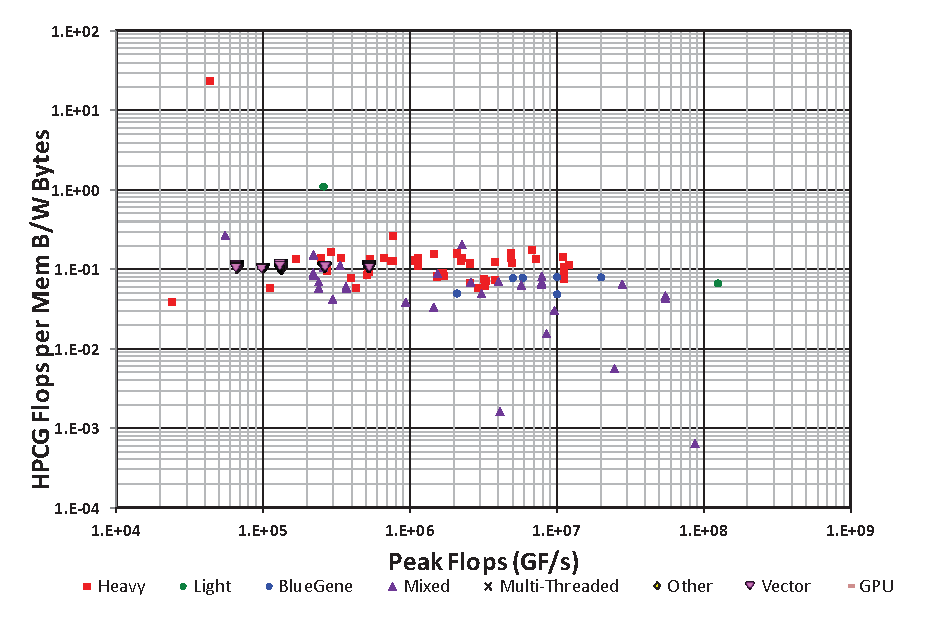
\includegraphics[scale=0.85]{../figures/spmv-historical-hpcg-bw.eps}
\caption{HPCG Flops per Byte of Memory Bandwidth vs. Peak flops.}
\label{fig:spmv-historical-hpcg-bw}
\end{centering}\end{figure*}

The HPCG benchmark \cite{techbib:hpcg-snl-dongarra} is one that is dominated time-wise by SpMV and similar kernels. Fig. \ref{fig:spmv-historical-hpcg-bw} diagrams data taken from recent HPCG reports\footnote{http://www.hpcg-benchmark.org/}. The x-axis is the peak flops of the reported system; the y-axis is the ratio of the sustained HPCG flops to the peak bandwidth of the systems's memory (derived by determining the processing chips used and looking up their characteristics). The color and shape refer to different types of chips and systems, with the red squares representing system built from server-class chips, and the purple representing system using GPUs. 

As can be seen, this ratio is independent of the peak system flops capability. In fact it is relatively flat at about 0.1 flops per byte of memory bandwidth for heavyweight server class processor chips, and somewhat less than 0.1 for GPUs and other architectures. Since SpMV is the bulk of HPCG, this is an indication that SpMV is relatively independent of core floating point capability, and instead highly dependent on chip memory bandwidth.

A recent complexity analysis of the HPCG benchmark \cite{techbib:marjanovic2014performance} dove into HPCG performance as a function of system parameter on a kernel-by-kernel basis. The particular implementation of HPCG that was studied assumed that a sub-matrix of the total matrix was processed in each MPI rank as executed by a single core. The study rolled these numbers up into total execution time for the whole benchmark as a function of just memory bandwidth and a few network parameters. The model was extremely accurate when compared to measured HPCG data on several benchmarks.

The analysis of just the SpMV kernel within HPCG focused on just the in-core time, and computed that each sub-row as executed by a single thread on a single core required a net of the following bytes fetched from memory\footnote{The paper computed a value of 27 for the average number of non-zeros per row partition, and each non-zero required two 8-byte fetches of floating point data and one 4-byte index reference, with another 20 bytes for starting the computation of a new row.}, where $nnz_{row}$ is the average number of non-zeros per row in the row as processed by each core:

\begin{equation}\label{eqtn:BytesPerRow}
20~+~20*nnz_{row}
\end{equation}

Since each non-zero represents two flops (an add and a multiply), dividing this into $2*nnz_{row}$ yields an estimate of the bytes of bandwidth needed from memory for each flop:

\begin{equation}\label{eqtn:BytesPerFlop}
2*nnz_{row}/(20~+~20*nnz_{row}) ~=~1/(10~+~10/nnz_{row})
\end{equation}

For a $nnz_{row}$ of 27 this is about 0.096 flops per byte of bandwidth. This correlates well with HPCG, as the non-SpMV parts of HPCG require slightly more bytes per flop. Approximately 10 bytes must be accessed from memory for each flops executed.

Multiplying this by the actual sustainable memory bandwidth of a node should then estimate the sustainable flops per second for SpMV running in all the cores in that node. \cite{techbib:marjanovic2014performance} uses in its projections the bandwidth number returned by using the Triad STREAM benchmark
%\cite{techbib:stream}. 
The first three rows of Table \ref{tab:analytic} summarize the characteristics of the three chips used in systems modelled by \cite{techbib:marjanovic2014performance}, including the ration of the reported STREAM bandwidth to the maximum memory bandwidth as projected by the chip's characteristics.


\begin{table*}\begin{centering}
  \centering
  \begin{tabular}{|c|c|c|c|c|c|c|c|c|c|c|c|}
\hline
&\multicolumn{4}{|c|}{Chip Parameters}&\multicolumn{4}{|c|}{Node Parameters}&\multicolumn{3}{|c|}{SpMV Specific}\\
\cline{2-11}
&&Total&Peak&Peak&&Peak&STREAM&&&Estimated&Measured\\
Chip&&Memory&B/W&Flops&&B/W&B/W&&&SpMV&SpMV\\
Type&Cores&Channels&(GB/s)&(GF/s)&Chips&(GB/s)&(GB/s)&Ratio&$nnz_{row}$&(GF/s)&(GF/a)\\
\hline\hline
\multicolumn{12}{|c|}{Chips used in Reference %\ref{techbib:marjanovic2014performance} 
	for HPCG Benchmark}\\ \hline
E5-2670&8&4&51.2&166.4&2&102.4&75.28&73.5\%&27&&\\ \hline
6276&16&4&51.2&147.2&2&102.4&54.4&53.1\%&27&&\\ \hline
X5560&4&3&32&44.8&2&64&27.44&42.9\%&27&&\\ \hline

\multicolumn{12}{|c|}{Chips used in Reference %\ref{techbib:6933066}
	 for SpMV Benchmark}\\ \hline
X5650&6&3&32&63.84&2&64&N/A&N/A&6.98&&1.9 \\ \hline
E5-2660&8&4&51,2&140.8&2&102.4&N/A&N/A&6.98&&5.3 \\ \hline


\multicolumn{12}{|c|}{Chips used in this paper.}\\ \hline
E5-2650v2&8&4&59.7&166.4 \\ \hline
\hline
  \end{tabular}
  \caption{SpMV Projection Based on System Parameters.}
  \label{tab:analytic}
\end{centering}\end{table*}
